% Chapter 1

\chapter{A Language of Polynomials} % Main chapter title

\label{Chapter1} % For referencing the chapter elsewhere, use \ref{Chapter1} 

%----------------------------------------------------------------------------------------

% Define some commands to keep the formatting separated from the content 
\newcommand{\keyword}[1]{\textbf{#1}}
\newcommand{\tabhead}[1]{\textbf{#1}}
\newcommand{\code}[1]{\texttt{#1}}
\newcommand{\file}[1]{\texttt{\bfseries#1}}
\newcommand{\option}[1]{\texttt{\itshape#1}}

%----------------------------------------------------------------------------------------

\section{Introduction}

This thesis is on the construction of the one way function to a matrix multiplication problem - that of multiplying two $3 \times 3$ matrices to form a $6 \times 6$ matrix under a locally concatenative property. The matrix multiplication is a type of law of composition that operates on different layers and although there are techniques to construct the multiplication of two $6 \times 6$ matrices, this paper examines the irreducible component of them. There may be some higher level mathematics mixed throughout the paper, however, thorough explanation will be attempted, otherwise can be ignored. The reason why it is included is to provide a bridge of multiple directions for the reader to take.

This paper aims to get the reader up to speed on the foundations of current computational complexity theory as it builds up a framework from scratch. At the end it provides a field for the reader to use in order to understand modern complexity theory in more depth. The intention is to provide as much insight as possible as to explore the science of computation.

%----------------------------------------------------------------------------------------

\section{Foundations}

There exists a language such that it decides each monomial in the polynomial. In other words, there exists a set of deciders for each monomial in the polynomial where it decides if y is in the monomial. A decider in this term is not of the definition found originally in textbooks but one that is redefined in the below definition.

$\newline$

Given a polynomial

$p(x) = ax^2 + bx + c$

$p(x) = 3x^2 + 4x + 5$

$p(2) = 3(2)^2 + 4(2) + 5$

$p(2) = 12 + 8 + 5$

$\newline$

Let the decider be defined as the following:

$\\ $

A monomial decider is a special kind of machine that decides if y is in a monomial. $Decider<c x^{n}> \equiv c x^{n} = y$ such that $x_1 \times x_2 \times ... \times x_n\ $ where $n$ is equal to $degree + constant$ of the monomial where $m(x) = cx^n$ and is tested to be equivalent to y. For each state, $q_i$, $i$ such that it is between 1 to n, $q_i$ contains a subgroup of size n and for each subgroup, $s_i$, there exists another subgroup and so on and so forth such that there are n layers. For each $s_i$, there is a start state, $q_{start}$ and a finish state, $q_{finish}$. This is the same as saying that it is a rational expression.

$\newline$

$\textbf{Examples}$

Decider for $ax^2$ is $Decider<3(2)^2> \equiv 3(2)^2 = 12$

Decider for $bx$ is $Decider<4(2)^1> \equiv 4(2)^1 = 8$

Decider for $c$ is $Decider<5(2)^1> \equiv 5(2)^0 = 5$

$\\ $

\begin{figure}[H]
  \centering
  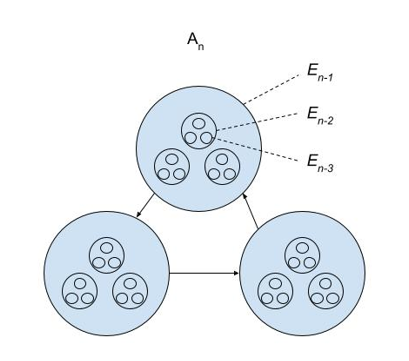
\includegraphics[scale=1]{0101DeciderX3.png}
  \caption{Decider that represents the monomial, $x^3$.}
  \label{fig:0101DeciderX3}
\end{figure}

\section{Monomial of One Variable}

Given the definition of a decider:

Decider is a function $Decider<cx^n>$ that tests if y is in $cx^n$.

$\\ $

A decider of at least one degree can be denoted as the following.

$Decider< 3 x^4 >$ that tests if y is in $3 x^4$.

$\\ $

Each state in the decider has monomials with the same property of being able to describe the lesser monomial which it contains and the following example is how it is denoted.

$\\ $

Contains $Decider<3 x^3> \equiv 3x^3 = y$

Contains $Decider<3 x_{0,j,2}^3>\cup \cdots\cup Decider<3 x_{2,j,2}^3>$

Contains $Decider<3 x_{0,j,1}^3>\cup \cdots\cup Decider<3 x_{2,j,1}^3>$

Contains $Decider<3 x_{0,j,0}^0>\cup \cdots\cup Decider<3 x_{2,j,0}^0>$

$\\ $

It can be generalized to:

$\\ $

$Decider<x_{0,j,1}^n>\subset \cdots \subset Decider<x_{i,j,k}^n>\subset \cdots \subset Decider<c x^{n}>$

such that i and j are the indices of the monomial representation and k is the layer the monomial representation is in.

$\\ $

It can be noted that there exists a start state, $q_{start}$ and a finish state, $q_{finish}$, for each semi-group in the decider. This has a more formal definition called a rational expression. A rational expression on A over K is a semi-ring described as $\mathcal{E}_{n}$ such that $n\geq0$ where A is an alphabet, in our case a finite set of integers, and K is a commutative semi-ring. This means the following in terms of the decider:

$\\ $

$Decider<c x^n>$ = $\mathcal{E}_{n}$

Contains $Decider<c x_{n-1}^n>\cup \cdots\cup Decider<c x_{n-1}^n>$ = $\mathcal{E}_{n-1}$

$\cdots$

Contains $Decider<c x_{2}^{n}>\cup \cdots\cup Decider<c x_{2}^{1}>$ = $\mathcal{E}_{2}$

Contains $Decider<c>\cup \cdots\cup Decider<c>$ = $\mathcal{E}_{1}$

$\\ $

The formal definition of a rational expression is defined below.

$\\ $

$\textbf{Definition 1.3.1. }$ $A_n = A_{n-1} \cup  {\left\{  E^* | E \in \mathcal{E}_{n-1}, (E,1)=0 \right\}}$

$\\ $

Here, $A_n$ is the set of monomials in the polynomial. $A_{n-1}$ are the monomials of degree n-1 and less of the polynomial and the set ${\left\{  E^* | E \in \mathcal{E}_{n-1}, (E,1)=0 \right\}}$ is equivalent to $Decider<cx^n>$ or equivalently the top of a single state of a decider. This theory has the opinion that it tries to describe finite recursion and nested for loops in a visual manner and, in so doing, this chain is chosen to be the best definition.

$\\ $

\begin{figure}[H]
  \centering
  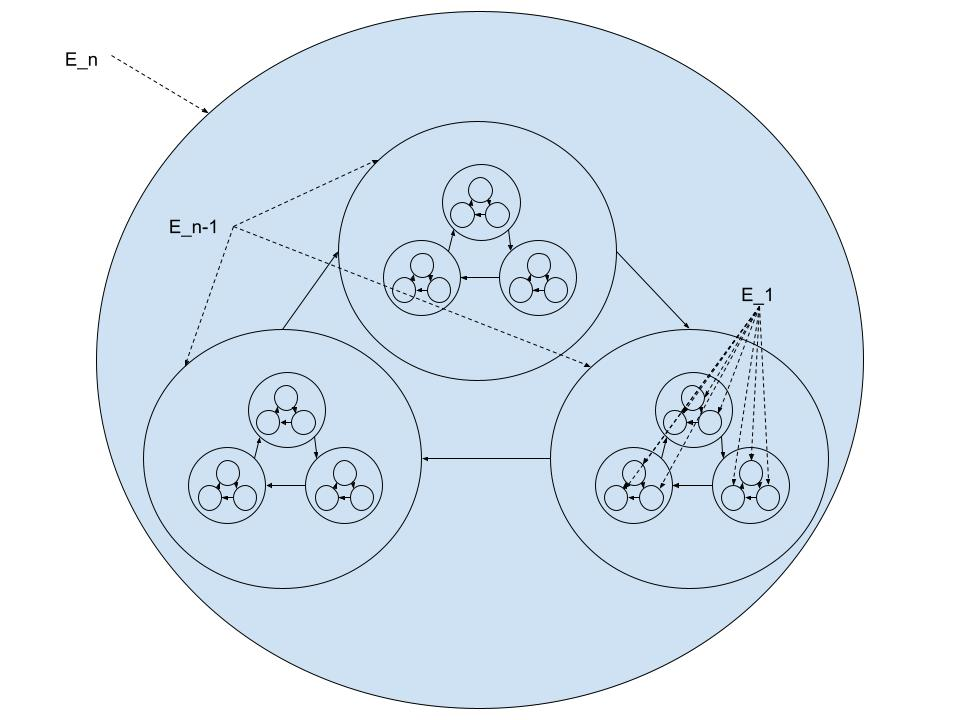
\includegraphics[width=\linewidth]{0103RationalExpression.jpg}
  \caption{Visual example of what $\mathcal{E}_n$ of a rational expression.}
  \label{fig:0103RationalExpression}
\end{figure}

$\\ $

A rational function is defined as the following: 

$\\ $

$\textbf{Defintion 1.3.2}$. K[[x]], or $K\ll A \gg$ is the set of functions that map a finite sequence, $A*$, to a semiring K of the alphabet, $A$, on the finite sequence, $A*$. Let K[[x]] describes a set of deciders as a polynomial representation. S is an element of K[[x]] meaning S is a polynomial decider.

$\\ $

S = $\sum_{n\geq 0}{a_n x^n}$

$\\ $

Unraveling a monomial decider can be reduced down to the layer $\mathcal{E}_1$. In the following proof of the theorem below, it can be noted that $q_{finish}$ isn't the same as $q\in q_{accept}$.

$\\ $

$\textbf{Theorem 1.3.3}$. A monomial decider represented as, $A_n$, can be mapped into a set consisting of the union of the base layer or $A_1 = \bigcup E_1$.

$\\ $

$\textbf{Corollary 1.3.4}$. A cyclic automata is in a monomial decider.

$\\ $

$\textit{Proof}$. For every $E_k$ in $A_n$, $E_k$ is a state that connects to $E_{k-1}$ where $1<k\leq n$.

For every $E_k$ to $E_{k-1}$, every semigroup of $q_{finish} \in E_1 \subset E_k$ connects to every other $q_{start}\in E_{k}$ forming a chain of cyclic semigroups.

Given $q_{finish}\in E_0$ in one semigroup connecting to another semigroup on $q_{start}\in E_k$, remove the connection and connect it to $q_{start}\in E_{k-1}$ where $1\leq k\leq n$ and n is a degree of the monomial.

This implies that $A_1 = \bigcup E_1$ hence it is a cyclic automata consisting of semigroups of $A_1$ that decides y on the monomial m(x).

$\\ $

\begin{figure}[H]
  \centering
  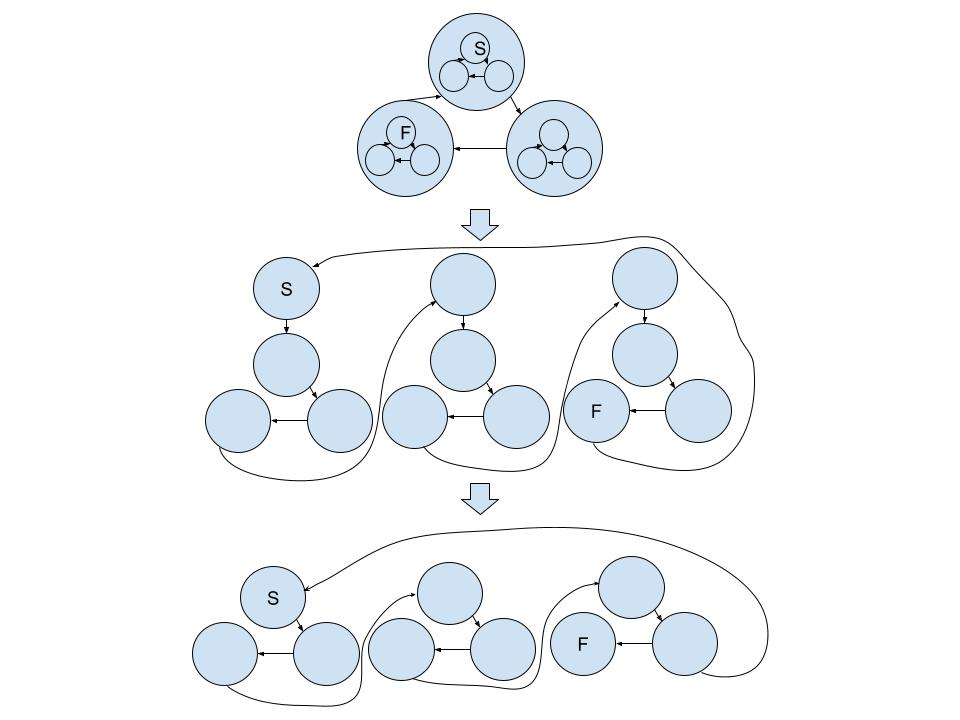
\includegraphics[width=\linewidth]{0102theorem.jpg}
  \caption{The unraveling theorem of a decider into a variant of cyclic automata.}
  \label{fig:0102theorem}
\end{figure}

$\\ $

The study of topology can describe the kind of space this variant of a decider forms.

$\\ $

A set X for which a topology $\tau$ has been specified is called a $\textbf{topological space}$. The following three properties are used as template to construct a decider.

$\\ $

$\textbf{Definition 1.3.5}$. A topology on a set X is a collection $\tau$ of subsets of $X$ having the following properties:

1. $\emptyset$ and $X$ are in $\tau$

2. The union of elements of any sub-collection of $\tau$ is in $\tau$

3. The intersection of the elements of any finite sub-collection of $\tau$ is in $\tau$

$\\ $

A decider is comprised of a start state and a finish state and some states that accept and others that reject. It can be null meaning that it is simply empty or it can be all the states. The union of some states gives a sub-collection of the topology of the decider which is a subspace of the topology of the decider. The intersection of the elements of the finite sub-collection of the topology of the decider is in the topology of the decider. Hence, this is the topology of a decider.

$\\ $

Furthermore, the types of states forming a decider can be described as a basis generating the decider seen in the following.

$\\ $

$\textbf{Definition 1.3.6}$. If $X$ is a set, a basis for topology on X is a collection $\textit{B}$ of subsets of $X$ such that:

1. For each $x \in X$, there is at least one basis element $B$ containing $x$

2. If $x$ belongs to the intersection of two basis elements $B_1$ and $B_2$, then there is a basis element $B_3$ containing $x$ such that $B_3 \subset B_1 \cap B_2$.

$\\ $

A decider has a start state, finish state, and two possible outcomes, accept and reject. It can be generalized that there are four kinds of states - start, finish, accept, and reject. These form a basis - $B_{start}$, $B_{finish}$, $B_{accept}$, and $B_{reject}$. Each basis element has at least one state. A state can be in the basis elements of start and accept, start and  reject, finish and accept, and finish and reject meaning that the intersection forms another basis element - the intersection of two basis elements. Thus, this is the topology of a decision function generated by $B_{start}$, $B_{finish}$, $B_{accept}$, and $B_{reject}$. 

$\\ $

A decider has an interesting property such that the space of each layer contained have the same property as the next layer below it until it reaches the base layer, $\mathcal{E}_1$.

$\\ $

$\textbf{Theorem 1.3.7}$. A monomial decider is a Hausdorff space.

$\\ $

$\textbf{Definition 1.3.8}$. A topological space X is called a Hausdorff space if for each pair $x_1$ and $x_2$ of distinct points X, there exist neighborhoods $U_1$, and $U_2$ of $x_1$ and $x_2$, respectively, that are disjoint.

$\\ $

$\textit{Proof}$. From $\textbf{theorem 1.3.3}$, a decider can be mapped into a cycle of states. If each state is a point, it is discrete and forms a neighborhood of the topology of the decider. Given two states, $q_i$ and $q_j$ such that $i\neq j$, the states are disjoint. Hence, by definition it is Hausdorff.

$\\ $

$\textbf{Theorem 1.3.9}$. A monomial decider has the property of being locally compact.

$\\ $

$\textbf{Definition 1.3.10}$. A space X is said to be locally compact at x if there is some compact subspace C of X that contains a neighborhood of x. If X is locally compact at each of its points, X is said simply to be locally compact.

$\\ $

$\textit{Proof}$. To show that a space is locally compact at a state, $q$, suppose that there is a subspace C of the topology of $A_n$ containing a neighborhood of $q$. This subspace is the topology of $E_1$. All subspace of the topology of $E_k$ such that $1<k\leq n$ contains $E_1$. Every state, $q$, of the topology of $E_k$ contains the subspace of the topology of $E_1$ thus $E_k$ is locally compact. Since $E_k$ is locally compact at every state, the topology of $A_n$ is locally compact.

$\\ $

$\textbf{Theorem 1.3.11}$. A monomial decider is a locally compact Hausdorff space.

$\\ $

$\textit{Proof}$. $A_n$ satisfies $\textbf{theorem 1.3.7}$ and $\textbf{theorem 1.3.8}$ hence it is locally compact and a Hausdorff space. Thus, it is a locally compact Hausdorff space.

$\\ $

\section{Addition}

\begin{figure}[H]
  \centering
  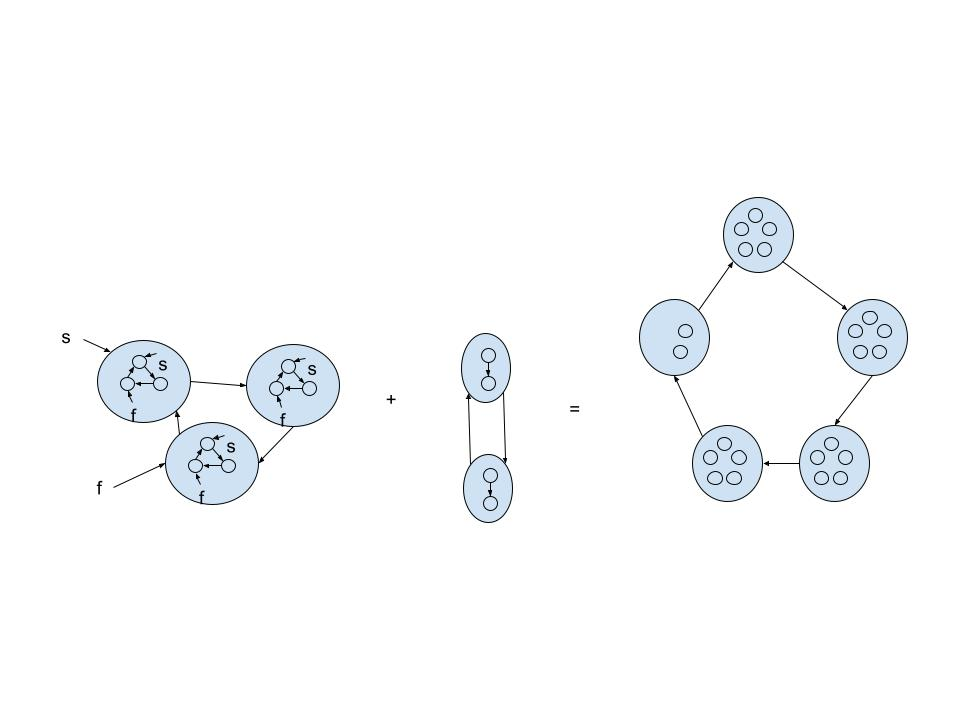
\includegraphics[width=\linewidth]{0104Addition.jpg}
  \caption{Addition of two deciders. The gradient of the circles remain the same after adding the two deciders together as the degree remains the same.}
  \label{fig:0104Addition}
\end{figure}

Each monomial in the polynomial can be tested in the decider and can be operated on by addition. 

$\\ $

$\textit{Example}$.

$m_1$ = $Decider<2 x^2>$ tests if y is in $2 x^2$.

$m_2$ = $Decider<4 x^4>$ tests if y is in $4 x^4$.

$\\ $

The following corollary of addition will be used to show a general theorem of addition.

$\\ $

$\textbf{Corollary 1.4.1}$. Given two monomials of the same degree, $m_1$ and $m_2$, the addition operation can be performed on them to form a decider of the aggregate, $m_3$, such that $m_3 = m_1 + m_2$.

$\\ $

$\textit{Proof}$. Using the unraveling theorem get to $E_1$ for the deciders on $m_1$ and $m_2$. Remove the connection on $q_{finish}$ to $q_{start}$ for both deciders. Connect $q_{finish}$ for the decider on $m_1$ on the layer $E_1$ to $q_{start}$ on the decider on $m_2$ on the layer $E_1$. Connect $q_{finish}$ on the decider on $m_2$ of $E_1$ to $q_{start}$ on the decider on $m_1$ of $E_1$. $q_{start}$ of the decider on $m_1$ is the new start start and $q_{finish}$ of the decider on $m_2$ is the new finish state of this new aggregate decider on $m_3$. Hence, this is the decider on $m_3$ which is the sum of $m_1$ and $m_2$.

$\\ $

The opposite is true which is splitting up the decider on $m_3$ to form $m_1$ and $m_2$.

$\\ $

$\textbf{Corollary 1.4.2}$. Given a monomial of some degree, $m_3$, it can be split up into two $m_1$ and $m_2$ such that $m_3 = m_1 + m_2$.

$\\ $

$\textit{Proof}$. Given a monomial, $m_3 = c x^n$, take $c = c_i + c_{i+1}$. Use the unraveling theorem to get the base layer, $\mathcal{E}_1$, on the decider on $m_3$. Group the states between $q_{start} to q_i$ of the decider on $m_3$ and set $q_i$ as the finish state of the new decider on $c_i x^n$. Then take the states between $q_{i+1}$ to $q_{finish}$ and set the start state of this new decider on $c_{i+1} x^n$ to $q_{i+1}$. Hence, these two constructions on the deciders of $c_i x^n$ and $c_{i+1} x^n$ form summation of the decider on $c x^n$.

$\\ $

These two corollaries can be generalized into algebra to form a theorem of addition.

$\\ $

$\textbf{Theorem 1.4.3}$. $Decider<c_1 x^n> + Decider<c_2 x^n> \equiv Decider<c x^n>$ such that $c = c_1 + c_2$.

$\textit{Proof}$. Given $m_1 = c_1 x^n$ and $m_2 = c_2 x^n$, there exists deciders on $m_1$ and $m_2$ denoted $Decider<c_1 x^n>$ and $Decider<c_2 x^n>$. Use the corollary of addition to form a decider on the aggregate of $m_1$ and $m_2$ called $m_3$ such that 

$m_3 = m_1 + m_2$

$=c_1 x^n + c_2 x^n$

$=(c_1 + c_2) x^n$

$=c x^n$

By definition, this is equivalent to $Decider<c x^n>$. For the reverse, take $c x^n$. Use the splitting corollary to get deciders on $c_i x^n$ and $c_{i+1} x^n$. Hence $Decider<c x^n>$ implies that it is equivalent to $Decider<c_i x^n> + Decider<c_{i+1} x^n>$.

\section{Product}

\begin{figure}[H]
  \centering
  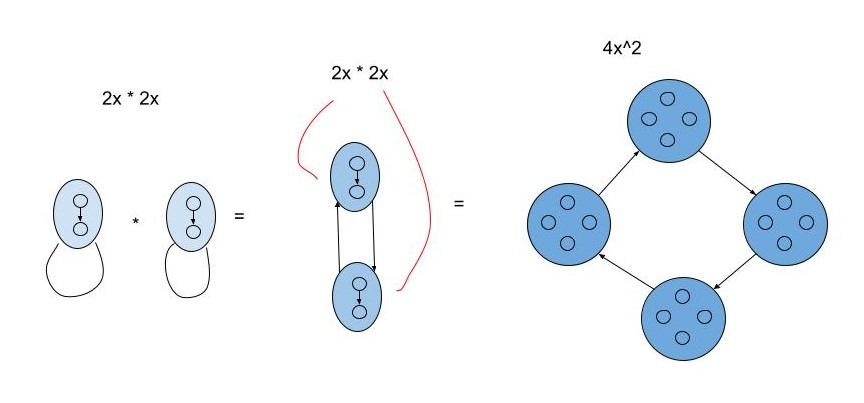
\includegraphics[width=\linewidth]{0105Product.jpg}
  \caption{Product of two deciders. The gradient of the circles get denser after adding the two deciders together as the degree increases.}
  \label{fig:0105Product}
\end{figure}

$\textbf{Theorem 1.5.1}$. $Decider<a x^m>$ * $Decider<b x^n>$ implies $Decider<c x^{m+n}>$ where $c = ab$.

$\\ $

$\textbf{Corollary 1.5.2}$. There is a decider on $x^n$ such that for every $\mathcal{E}_k$ where $1\leq k\leq n$, for every semigroup in $\mathcal{E}_k$, there is n semigroups in $\mathcal{E}_k$ is equivalent to the topology of the decider on $x^n$ being a locally compact Hausdorff space.

$\\ $

$\textit{Proof}$. Suppose $A_n$ is the decider on $x^n$ then there are n semigroups in $\mathcal{E}_k$ for all k in the closed set $[1,n]$. These semigroups form a subspace of the topology of the decider on $x^n$ by definition implying that the union of these n subspaces form a topology that it is a locally compact Hausdorff space. 

$\\ $

Suppose the reverse is true, that the topology on the decider on $x^n$ is a locally compact Hausdorff space. There are n subspaces whose union form the topology of the decider on $x^n$ at $\mathcal{E}_k$. These subspaces are equivalent to a semi-group because they can be added together by the corollary of addition at any layer, $\mathcal{E}_k$, and they have the identity of itself. Since every subspace on $\mathcal{E}_k$ is a locally compact Hausdorff space this implies that every semi-group contains n semi-groups for every $\mathcal{E}_k$.

$\\ $

Now, given $Decider<c_x x^m>$ and $Decider<c_y x^n>$, show that the product is $Decider<(c_x c_y) x^{m+n}>$. It can be seen that there are $m$ and $n$ layers for the deciders on $c_x x^m$ and $c_y x^n$, respectively. When multiplied together, this results in $m+n$ layers. Construct a new decider from the the two deciders given to get $Decider<(c_x + c_y) x^{m+n}>$ by operating at the highest level, $\mathcal{E}_{n}$ and using the corollary above. Hence, $Decider<c_x x^m>$ multiplied by $Decider<c_y x^n>$ gives us the product, $Decider<(c_x+c_y) x^{m+n}>$.

\section{A Conjecture with Matrices}

An important problem arising from deciders is representing them as matrices. The problem can be reformulated as the following: given a polynomial, show that the monomials represented in the language can't be contained in a finite matrix after a set number, n, such that $x^n$. Equivalently, multiplying two matrices together gives the product of a matrix whose dimensions are greater than the dimensions multiplied by. The conjecture can be stated below.

$\\ $

$\left[ n\times n \right]\left[ n\times n \right]=\left[ m\times m \right]$ such that $0< n< m$

$\\ $

The focus of this article pertains to the question of whether or not there exists structures with certain properties that allow law of compositions to handle the above statement. The reason why this seems feasible is because of the following proposition found in Retenaur(66).

$\\ $

$\textit{Proposition.}$ Given a proper square matrix M over $\mathcal{E}$, there exist matrices $M_1$, $M_2$ of the same size as M over $\mathcal{E}$ such that $M_1 ~1 + MM_1$ and $M_2~1+M_2M$. In particular if K is a ring, 1 - M is an invertible modulo ~.

$\\ $

If this is true, there is are techniques that exist to reduce $M_1$ and $M_2$ into irreducible elements and have them mapped into visually format in order to understand the operation at a higher level.

\section{Generalized Monomial Deciders}

\begin{figure}[H]
  \centering
  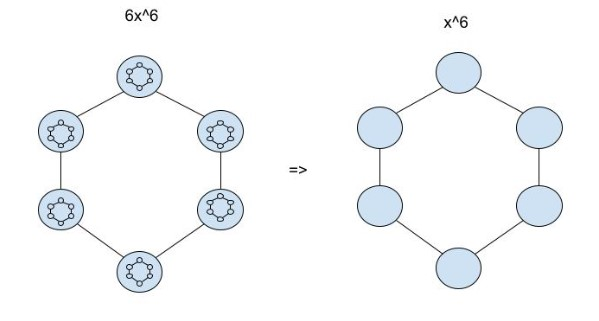
\includegraphics[scale=1]{0107Generalized.jpg}
  \caption{Generalization of a monomial decider.}
  \label{fig:0107Generalized}
\end{figure}

A decider can be represented as the top layer only if short hand notation is necessary. In a way, this removes the constant which is a term called being $\textit{proper}$. Given a Decider<m(x)> where m(x) is a monomial, keep the top layer $S_n$ in $\mathcal{E_n}$. This is called the generalized monomial decider. This representation will be used in order to keep deciders simple but it doesn't remove the property of \textbf{corollary 1.5.2}.

\section{Constants}

\begin{figure}[H]
  \centering
  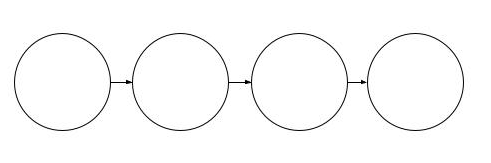
\includegraphics[scale=1]{0109Constants.png}
  \caption{A constant represented as decider.}
  \label{fig:0109Constants}
\end{figure}

Representing a constant can be seen as a set of acyclic graphs. Given a constant, c, of a polynomial: f(x) = c, there exists a linear directed acyclic graph to represent the constant visually.

$\\ $

Addition gives the following:

$Decider<c_1 x^0> + Decider<c_2 x^0>$ 

$ = Decider<(c_1+c_2) x^0>$ by $\textbf{corollary 1.4.1}$

$ = Decider<c_1 + c_2>$ since $x^0$ is the identity

$\\ $

There is no state in the decider where it loops back to the start. The constant is what separates a decider from a strictly mathematical cyclic object, semi-simple groups. In software engineering, most programs are written in way to make it have a logical flow of that being a linear logical chart. In this way, many programmers can understand the program better and it keeps the code organized.

\section{Division}

There are a finite amount of permutations, called decision functions, in a decider.

$\\ $

\begin{figure}[H]
  \centering
  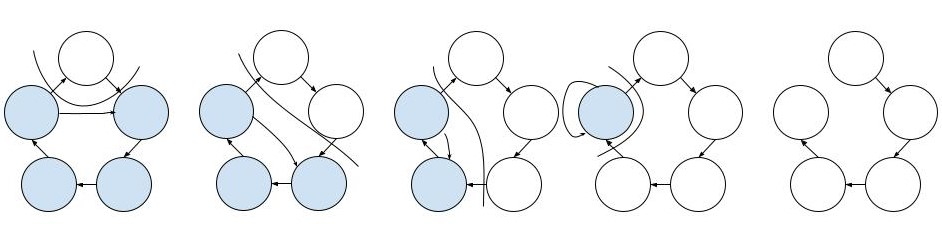
\includegraphics[width=\linewidth]{0110x5.jpg}
  \caption{One decision function of $Decider<x^5/x>$ to one decision function of $Decider<x^5/x^5>$.}
  \label{fig:0110x5overx}
\end{figure}

In order to show the number of decision functions in a decider, start with the a formula to calculate the amount of permutations given some integer, $n$, and the number of spaces, or partitions, being permuted. $\textbf{Theorem 1.9.1}$ and $\textbf{corollary 1.9.2}$ is found in Rosen (407). 

$\\ $

$\textbf{Theorem 1.9.1}$. If $n$ is a positive integer and $r$ is an integer with $1\leq r \leq n$, then there are

$P(n,r) = n(n-1)(n-2)\cdots (n-r+1)$

r-permutations of a set with $n$ distinct elements.

$\\ $

The following corollary is derived from the theorem.

$\\ $

$\textbf{Corollary 1.9.2}$. If $n$ and $r$ are integers with $0\leq r\leq n$, then $P(n,r)$ = $\frac{n!}{(n-r)!}$.

$\\ $

Now, on a single division operation, two spaces are split into two, the original and the space divided. This implies the following corollary.

$\\ $

$\textbf{Corollary 1.9.2}$. On a single operation, there are two distinct spaces formed on a decider on $x^n$ giving $n(n-1)$ decision functions on the space of the decider.

$\\ $

$\textit{Proof}$. There are two spaces being permuted showing that r is 2. By $\textit{theorem 1.9.1}$, this gives $\frac{n!}{(n-2)!}$ = $n(n-1)$ permutations on the space of the decider on $x^n$.

$\\ $

$\textit{Example}$. The following denotations are deciders related to $x^5/x^i$ such that $1 \leq i \leq 5$.

$m_1 = Decider<x^5>/Decider<x^1>$

$m_2 = Decider<x^5>/Decider<x^2>$

$m_3 = Decider<x^5>/Decider<x^3>$

$m_4 = Decider<x^5>/Decider<x^4>$

$m_5 = Decider<x^5>/Decider<x^5>$

$\\ $

\section{Multiple Divisions}

\begin{figure}[H]
  \centering
  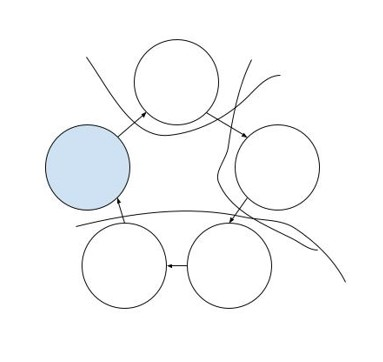
\includegraphics[width=\linewidth]{0111MultipleDivisions.jpg}
  \caption{$Decider<x^5/x/x/x^2>$}
  \label{fig:0111MultipleDivisions}
\end{figure}

$\\ $

Generalizing to multiple operations on the decider on $x^n$, a corollary can be derived.

$\\ $

$\textit{Corollary 1.11.1}$. On multiple operations of division, the number of permutations of the space on $x^n/Q$ where $q_i\in Q$ such that $1\leq i\leq n$ is equal to $\frac{n}{(n-r)!}$ by $\textbf{corollary 1.9.2}$.

$\\ $

The topology of the decider on $x^n$ can be formed.

$\\ $

A decider of a monomial forms a space having no decision functions or the set of all decision functions so $\emptyset \in \tau$ or $D \subseteq \tau$. These aren't included in the calculations of the permutations a decision function can have as there is no division operations being performed.

$\\ $

The union of sets of decision functions, $D$, of $\tau$ is in $\tau$.

$\\ $

$d_1, d_2 \in D \subseteq \tau$ such that $d_1 \cup d_2 \subseteq D \subseteq \tau$ implies $d_1, d_2 \in \tau$.

$\\ $

The intersection of sets of decision functions, $D$, of $\tau$ is in $\tau$. 

Given $d_1 \in D_1$ and $d_1 \in D_2$, then $d_1 \in D_1 \cap D_2 \subseteq \tau$.

$\\ $

Using the construction above, another layer of topology of a decider is formed to find in order to find general patterns latter in this paper.

$\\ $

The topology of the operations on the cyclic structure of a decider forms its own area of study. A topology of a decider used in this paper is constructed below. A basis that can be formed is one that describes the operations on $x^{n+k}/Q$ where Q is the divisions (e.g. $x^6/q_1/q_2$ where $q_1,q_2\in Q$). There are $6(6-1)(6-2)$ = $120$ permutations possible in the example given. The basis elements that form $B_{q_1 q_2}$ and $B_{q_2 q_1}$ can be described. As a programmer, this statement means that even though there are many ways to write a function, there a finite amount of different combinations to write them in terms of having be as re-factored well.

$\\ $

$\textit{Example}$. The following are examples on $x^n/Q$

$Decider<x^5/x^2/x/x>$.

$Decider<x^5/x^2/x^2>$.

$Decider<x^5/x^2/x^1/x^1>$.

$Decider<x^5/x^2/x^2>$.

\section{Multivariable Monomials}

\begin{figure}[H]
  \centering
  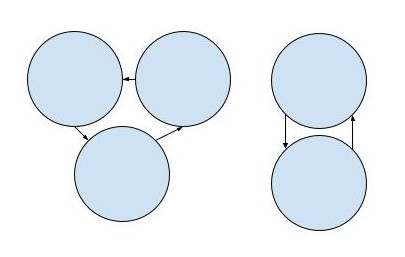
\includegraphics[scale=1]{0106Multivariables.jpg}
  \caption{Multivariable monomial deciders can be seen treated as parallel processes running next to each other.}
  \label{fig:0106Multivariable}
\end{figure}

A monomial with more than one variable can be treated the same way as handling single variables at different degrees by separating them out into a series to form an function. This function is called a rational function when division is taken into account.

$\\ $

Given a series of variables, $v_1,\cdots ,v_n$, a series of deciders can be constructed to decide each variable. 

$\\ $

$S = \sum_{i\geq 1}{v_i}$

$\\ $

A rational series on K[[x]] is a commutative ring on K consisting of an alphabet with a single letter x.

$\\ $

$\textbf{Definition 1.12.1}$ A rational series on K[[x]] denoted as

$\\ $

$R(x) = \sum_{n\geq 0}{a_n x^n}$

$\\ $

Each variable in $v_1,\cdots ,v_n$ is can be treated as to $v_i$ = $a_i x^i$. This means the following.

$\\ $

$\textbf{Theorem 1.12.2}$. A rational series, $R(x)$ can be decided by a decider on $R(x)$.

$\\ $

$\textit{Proof}$. TODO

\section{Equivalence}

\begin{figure}[H]
  \centering
  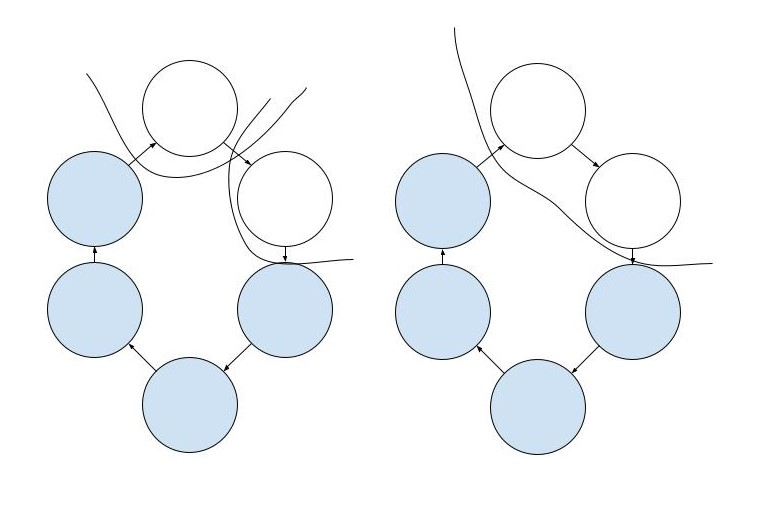
\includegraphics[width=\linewidth]{0112Equivalence.jpg}
  \caption{$Decider<x^6/x^2>$}
  \label{fig:0112Equivalence}
\end{figure}

$Decider<x^6/x^1/x^1> ~ Decider<x^6/x^2>$

$\\ $
Determining if y is in f x is easy if we are given any monomial decider in the set of the language of polynomials and their representations has the possibility to give different representations if we consider them as representations of the function f of x.

$\\ $

$Decider<x^6/x^1/x^1> \sim Decider<x^6/x^2>$ in that they decide if y is in m(x) = $x^6/Q$

$\\ $

$\textbf{Theorem of Equivalence}$. Something on lines of $Decider<x^6/x^1/x^1> = Decider<x^6/x^2>$ such that there is some x such that the monomial represented by both deciders exists where f of x = y.

$\\ $

$\textit{Proof}$. Given $Decider<a(x,y)> = Decider<x^m> Decider<y^n>$ and the definition $Decider<b(x,y)> = Decider<y^n> Decider<x^m>$, show $Decider<a(x,y)> = Decider<b(x,y)>$.

$\\ $

Start with $Decider<a(x,y)> = Decider<x^m> Decider<y^n>$

Commute the variables because each decider decides there own monomial giving, $Decider<y^n> Decider<x^m>$.

This is equivalent to $Decider<b(x,y)>$

$\\ $

Start with $Decider<b(x,y)> = Decider<y^m> Decider<x^n>$

Commute the variables because each decider decides there own monomial giving, $Decider<x^n> Decider<y^m>$.

This is equivalent to $Decider<a(x,y)>$

\section{Reversing}

$\\ $

$Decider<x^6/x^1/x^1> \equiv $sequence of permutations such that it is equal to $\sum_{i}^{n-1}{i}$

$\\ $

$Decider<x^6/x^2> \equiv $ sequence of permutations of $x_i$, $x_j$ such that it equals n-1.

$\\ $

Is shown that by the permutation of the order of operations that $Decider<x^6/x^1/x^1>$ does not have the same number of permutations as $Decider<x^6/x^2>$

$\\ $

$\textbf{Theorem of Reversing}$. Given two representations, a,b in $Decider<m(x)/Q>$ where m(x) is monomial and Q is the division operations such that m(x)/Q $\geq $ 1, a != b implies that they don't have the same quotients space.

$\\ $

$\textit{Proof}.$ Given $Decider<a(x,y)> = Decider<x^m> Decider<y^n>$ and the definition $Decider<b(x,y)> = Decider<y^n> Decider<x^m>$, show $Decider<a(x,y)> \neq Decider<b(x,y)>$.

$\\ $

Start with $Decider<a(x,y)> = Decider<x^m> Decider<y^n>$. 

Then take $Decider<x^m y^n>$. 

Commute to get $Decider<y^n x^m>$.

This is not equivalent to $Decider<y^n> Decider<x^m> = Decider<b(x,y)>$.

$\\ $

Start with $Decider<b(x,y)> = Decider<y^n> Decider<x^m>$.

Then take $Decider<y^n x^m>$

Commute to get $Decider<x^m y^n>$

This is not equivalent to $Decider<x^m> Decider<y^n> = Decider<a(x,y)>$

\begin{figure}[H]
  \centering
  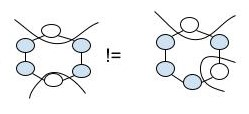
\includegraphics[scale=1]{0113Reversing.jpg}
  \caption{Two possible representations of $Decider<x^6/x/x>$.}
  \label{fig:0113Reversing}
\end{figure}

The two representations in 1.13 don't have the same quotient space and hence a != b.

\section{Corollary of Reversing}

Given a starting point of decider, the path the decider takes to decide if y is in the monomial, m(x) is unique to each representation. 

$\\ $
$\textbf{Corollary}$. Given a decider, d, in $Decider<m(x)>$ then there is path, p, that exists for d such that p = Path(d) = $s_1,s_2,...,s_i,...,s_n$ where i is count of the states in the decider of m(x).

$\\ $

$\textit{Example}$. Choose some x such that it is in path of $Decider<x^6/x^2>$ where $p = 001111$ then the following graph is what the decider is represented as.

\begin{figure}[H]
  \centering
  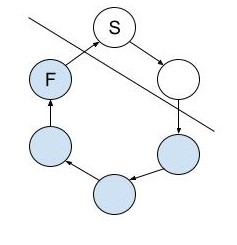
\includegraphics[scale=1]{0114CorollaryOfReversing.jpg}
  \caption{Path of one representation of $Decider<x^6/x^2>$.}
  \label{fig:0114CorollaryOfReversing}
\end{figure}

\section{Godel's Theorem}

We see that there exists two statements from these theorems

$\\ $

1. $x = x$ from a theorem of equivalence

2. $x != x$ from a theorem of reversal

$\\ $

$\textbf{Example}$: Given some $d_1$,$d_2$,$d_3$,...,infinity in decision functions in $Decider<m(x)>$

$\\ $

1. $d_1 = d_2 = d_3 = ... = infinity$

2. $d_1 != d_2 != d_3 = ... != infinity$

$\\ $


\begin{figure}[H]
  \centering
  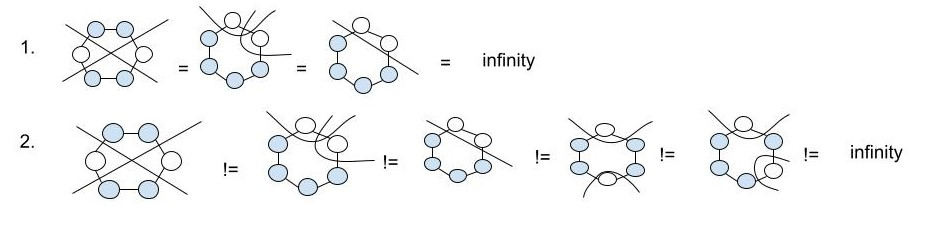
\includegraphics[width=\linewidth]{0115Godels.jpg}
  \caption{Godel's illustrated from $Decider<x^6/x^2>$.}
  \label{fig:0115Godels}
\end{figure}

$\\ $

The different representations of a monomial through the language of monomial deciders will give the problem of undecidability. This means that despite many formal definitions of the monomial decider, there is no way to solve the problem of finding a specific representation of a monomial decider without having to guess or apply some sort of probability to it. Relating to the real line, given a real line a,b a $\leq$ b, there is infinite choices between a and b. As long as b and a $\geq $ 0, there requires some sort of probability of choosing some specific number that is between a and b.

\section{Constructing The One Way Function}

A probability exists to find a certain monomial decider in the set of it's variations. A/B = Probability where A is the monomial decider we want and B is the number of all the variations.

$\\ $

$\textit{Example}$: $d_1$,$d_2$,...,$d_6$ in $Decider<x^6>$ such that $d_i$ are all distinct. 

Choose one of the deciders in D through probability

Probability of choosing d in D is 1/6 so 0.16666667

\begin{figure}[H]
  \centering
  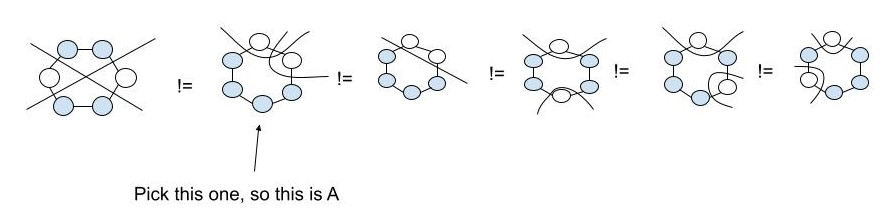
\includegraphics[width=\linewidth]{0116Constructing.jpg}
  \caption{Picking a decision function, d, from $Decider<x^6/x^2>$.}
  \label{fig:0116Constructing}
\end{figure}


$\\ $

This is called the picking function and every time it is called, the probability is multiplied such that it is $n^k$. As an example, if the picking function is called twice using the example above, it is shown that the probability is:

$1/6 \times 1/6 = 1/6^2 = 1/36 = 02777778$

$\\ $

This is formally known as the one way function.
